\documentclass[tikz,border=3pt]{standalone}
\usepackage[utf8]{inputenc}
\usepackage[T1]{fontenc}
\usepackage{lmodern}
\renewcommand{\familydefault}{\sfdefault}
\usepackage{sansmath}\sansmath
\usepackage{pgfplots}\pgfplotsset{compat=1.18,/pgf/number format/use comma,/pgf/number format/1000 sep={.}}
\usetikzlibrary{arrows.meta,calc,positioning,decorations.pathmorphing,patterns}
% paleta del sitio
\definecolor{nar}{HTML}{E8680C}\definecolor{narc}{HTML}{FFB35C}\definecolor{hielo}{HTML}{FFF3E8}
\definecolor{tinta}{HTML}{1D1D1F}\definecolor{gris}{HTML}{6E6E73}\definecolor{lila}{HTML}{7C5CF0}
\definecolor{azul}{HTML}{2F6FD6}\definecolor{menta}{HTML}{17A673}\definecolor{coral}{HTML}{E8342A}
\begin{document}
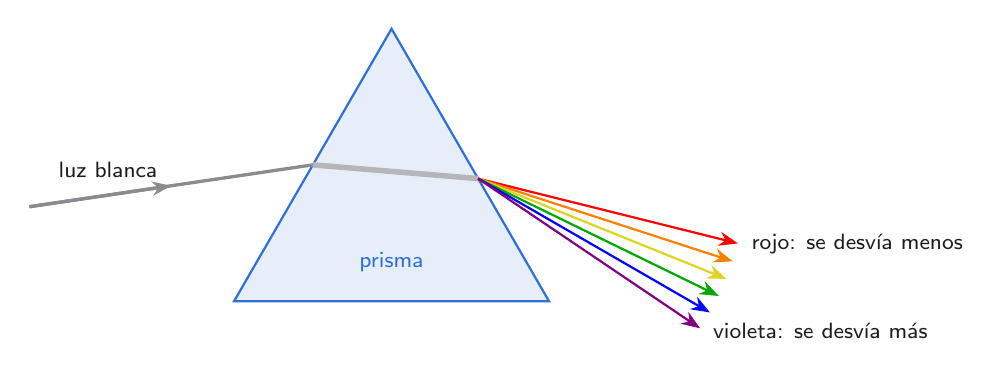
\begin{tikzpicture}[font=\footnotesize,>={Stealth[length=2.4mm]}]
\fill[azul!12,draw=azul,thick] (0,0) -- (4,0) -- (2,3.46) -- cycle;
\draw[very thick,gris!80] (-2.6,1.2) -- (1,1.732);
\draw[->,very thick,gris!80] (-2.6,1.2) -- (-0.8,1.466);
\node[above,text=tinta] at (-1.6,1.45) {luz blanca};
\draw[line width=2pt,gris!50] (1,1.732) -- (3.1,1.557);
\foreach \c/\ang in {red/-14, orange/-18, yellow!85!black/-22, green!65!black/-26, blue/-30, violet/-34}
  \draw[->,thick,\c] (3.1,1.557) -- ++(\ang:3.4);
\node[right,text=tinta] at ($(3.1,1.557)+(-14:3.45)$) {rojo: se desvía menos};
\node[right,text=tinta] at ($(3.1,1.557)+(-34:3.45)$) {violeta: se desvía más};
\node[text=azul] at (2,0.5) {prisma};
\fill[white] (6.5,-0.75) circle (0.01);
\end{tikzpicture}
\end{document}
